\section{Étude de convergence}

Afin d'évaluer au mieux l'amélioration apportée par l'utilisation des splines d'Hermite, il est intéressant de comparer
les résultats rendus par les éléments quadratiques d'une part et les splines d'Hermite d'autre part et ce pour la
méthode classique et la méthodes basée sur les caractéristiques.

La convergence des différentes méthodes est évaluée en utilisant la formule d'erreur proposée en~\eqref{FEM1D:errf}.
Les résultats sont présentés en figure~\ref{fig:comp_quad_herm} qui permet de comparer plusieurs configurations.

\begin{figure}[!ht]
	\centering
	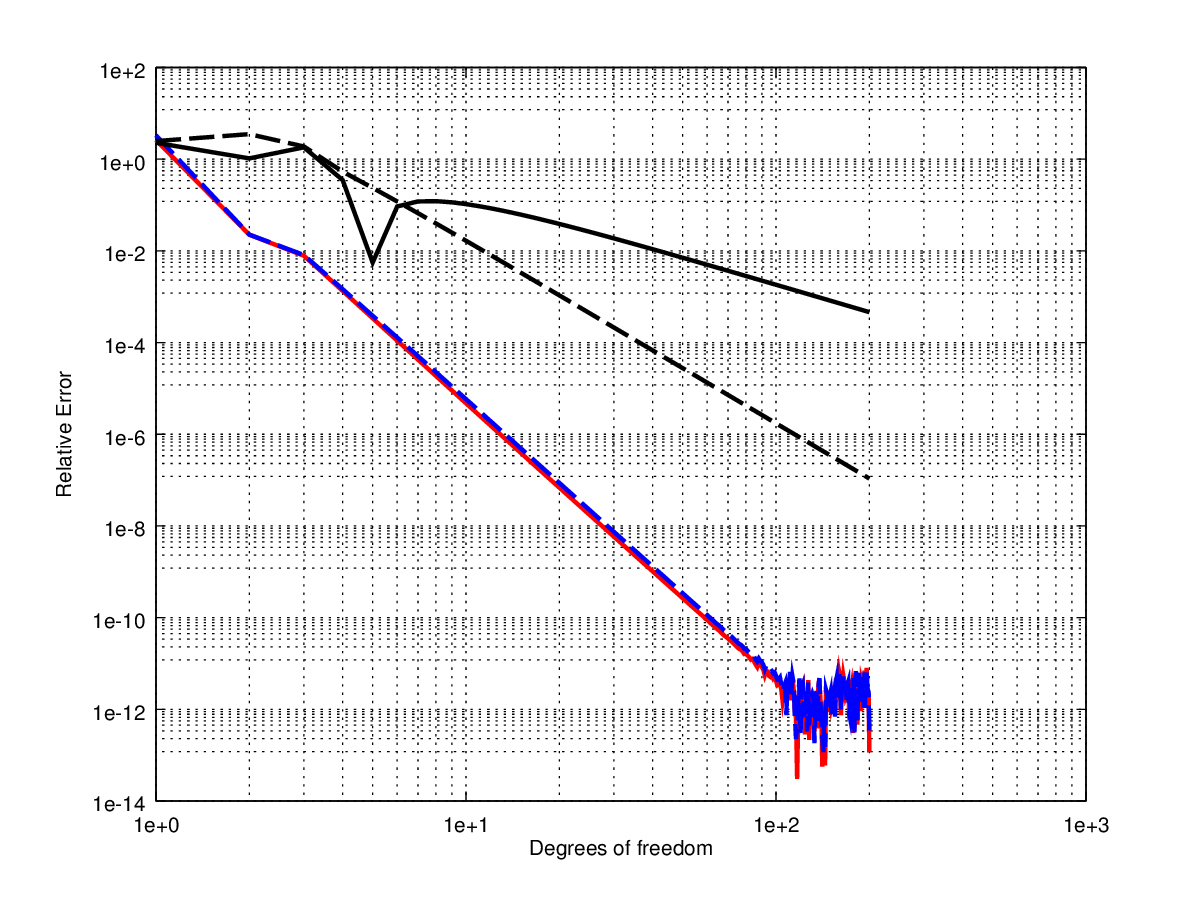
\includegraphics[width=11cm]{part4/figs/herm_comp.png}
	\caption{\label{fig:comp_quad_herm}Erreur relative commise avec des éléments quadratiques en noir (tireté,
	méthode classique ; plein, méthode des caractéristiques) et avec des splines d'Hermite (en rouge et bleu).}
\end{figure}

\paragraph{Entre éléments quadratiques et splines d'Hermite}
Dans tous les cas, les splines d'Hermite donnent de meilleurs résultats que les éléments quadratiques. Les courbes de
convergence pour les méthodes basées sur des splines ont, en effet, un ordre de pente supplémentaire par rapport aux
éléments quadratiques. De ce point de vue au moins, le passage à des splines d'Hermite est un gain.

\paragraph{Entre méthode classique et méthode par caractéristiques}
Alors que pour des éléments quadratiques la méthode classique convergeait plus vite, pour les splines d'Hermite, ce
n'est pas le cas.
Le fait de pouvoir immédiatement accéder à la dérivée de la pression comme inconnue du problème permet de s'affranchir
de la perte d'un ordre de convergence lors du passage aux caractéristiques. Les résultats entre la méthode classique et
la nouvelle méthode proposée pour une interpolation des champs par splines d'Hermite ont exactement la même alors. Si
les courbes pour ce système d'interpolation sont observées de plus près (voir figure~\ref{fig:herm_seul}), il est
notable que la courbe de convergence pour la méthode par caractéristiques est d'ailleurs en dessous de celle pour la
méthode classique, ce qui suggère une erreur plus faible.

\begin{figure}[!ht]
	\centering
	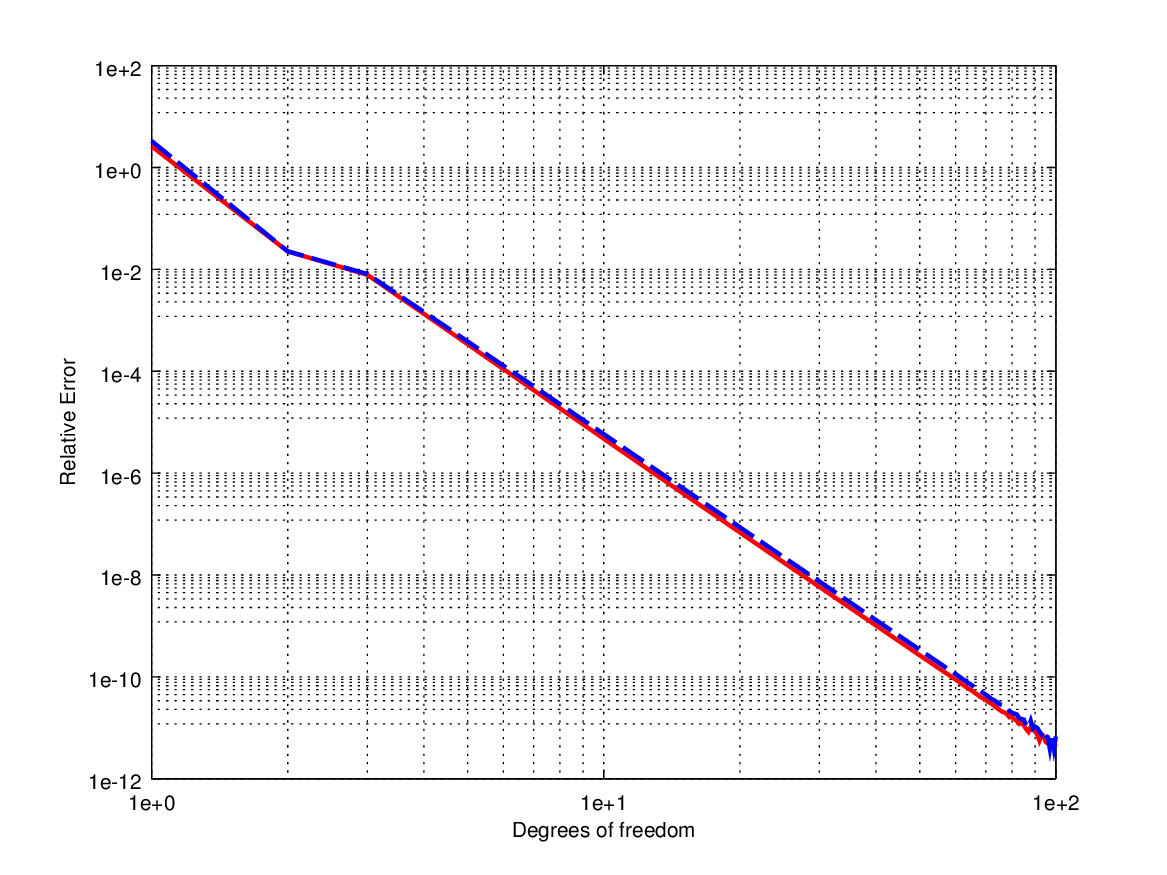
\includegraphics[width=11cm]{part4/figs/herm_seul.png}
	\caption{\label{fig:herm_seul}Erreur relative commise avec des splines d'Hermite (en rouge méthodes des
    caractéristiques et en bleu, méthode classique).}
\end{figure}
